\section{Difracción}
\rfigure
% \setcounter{equation}{0}
%
\pma{\label{p:P231}
Considere un haz de ondas planas que incide sobre una placa que contiene una rendija. Si la intensidad del máximo central en el patrón de difracción es $I_\text{max}$, determine la intensidad (relativa a la máxima) de los primeros 3 máximos secundarios de difracción.\\
\rta{.95}{$I_1=0.047\,I_\text{max}$, $I_2=0.016\,I_\text{max}$, $I_3=0.008\,I_\text{max}$}
}
%
\pma{\label{p:P237}
Los rayos paralelos de un haz de luz de longitud de onda $\lambda_0=650$~nm pasan por una pantalla en la cual se halla una rendija de $0.5$~mm de ancho y 3~cm de alto. El patrón de difracción generado por esta rendija se observa en una pantalla ubicada 50~cm a continuación de la rendija. Calcular la distancia, medida sobre la pantalla, entre el máximo principal del patrón de difracción y \textit{a}) los primeros mínimos, \textit{b}) los primeros máximos secundarios.\\
\rta{.95}{\textit{a}) $\pm0.65$~mm; \textit{b}) $\pm0.93$~mm}}
%
\pma{\label{p:P238}
Se observa el patrón de difracción generado por una rendija de $0.25$~mm de ancho sobre una pantalla situada a una distancia de $2.5$~m de ella. La campana principal de difracción tiene un ancho de 11~mm. ¿Cuál es la longitud de onda de la luz utilizada?\\
\rta{.95}{550~nm}
}
%
\pma{\label{p:P239}
Se ilumina con luz infrarroja proveniente de un láser de He-Ne ($\lambda_0= 1152.2$~nm en el vacío) una pantalla que contiene una rendija estrecha, y se determina que el centro de la décima banda oscura en el patrón de difracción de Fraunhofer se encuentra en un ángulo de $\SI{6.3}{\degree}$ respecto del eje central. \textit{a}) Calcule el ancho de la rendija. \textit{b}) ¿Para qué ángulo aparecerá la décima franja oscura si todo el arreglo se sumerge en agua $\left(n_a(\lambda_0) = 1,326\right)$ en lugar de aire?\\ \rta{.95}{\textit{a}) $a=\SI{105}{\micro\meter}$; \textit{b}) $\theta_{10}=\SI{4.747}{\degree}$}}
%
\pma{\label{p:P240}
Calcule el ancho $a$ de la ranura rectangular que producirá en su patrón de difracción de campo lejano una campana principal con un ancho angular $\delta\theta$ de \textit{i}) $\SI{30}{\degree}$, \textit{ii}) $\SI{45}{\degree}$, \textit{iii}) $\SI{90}{\degree}$, \textit{iv}) $\SI{180}{\degree}$, al ser iluminada con de longitud de onda 550~nm.\\
\rta{.95}{\textit{i}) $\SI{2.125}{\micro\meter}$; \textit{ii}) $\SI{1.437}{\micro\meter}$; \textit{iii}) $\SI{0.778}{\micro\meter}$; \textit{iv}) $\SI{0.550}{\micro\meter}$}}
%
\pma{\label{p:P241}
El patrón de difracción producido por una única rendija, cuando se la ilumina con luz de 550~nm, es observado sobre una pantalla ubicada a 40~cm a continuación de la placa que contiene a la rendija. Si la distancia entre el primer y quinto mínimo es de $0.4$~mm, determinar el ancho de la rendija.
\rta{.95}{\textit{a}) $a=2.2$~mm}}
%
\begin{minipage}[t]{.5\textwidth}
  \textbf{Pantallas complementarias}. Consideremos dos superficies $\Sigma$ y $\Sigma'$ de manera tal que en los puntos donde la superficie $\Sigma$ es transparente, $\Sigma'$ es opaca y viceversa, como se muestra en la figura \ref{f:babinet}. Por ejemplo, si $\Sigma$ es un agujero circular en una pantalla opaca, entonces $\Sigma'$ es un disco opaco del mismo tamaño y posición en una pantalla transparente. Este tipo de pantallas se denominan complementarias. Se puede mostrar que el patrón de difracción de la pantalla $\Sigma$ es el mismo que produce la pantalla $\Sigma'$ (salvo en la dirección de la onda incidente). Este hecho se conoce con el nombre de \textit{principio} o \textit{teorema de Babinet}.
\end{minipage}
\hfill
%\begin{figure}
\begin{minipage}[t]{.55\textwidth}
\strut\vspace*{-\baselineskip}

  \pgfdeclarelayer{layer1}
  \pgfdeclarelayer{layer2}
  \pgfdeclarelayer{layer3}
  \pgfsetlayers{main, layer3, layer2, layer1}

  \begin{center}
  \begin{tikzpicture}[x={(1cm,0.4cm)}, y={(8mm, -3mm)}, z={(0cm,1cm)}, line cap=round, line join=round, scale=0.75]
    \begin{pgfonlayer}{layer1}
      \object{3}
      \ray(0,-1,0)(2.5,-1,0)(0.5)(1);
      \ray(0,1,0)(2.5,1,0)(0.5)(1);
    \end{pgfonlayer}
    \begin{pgfonlayer}{layer3}
      \image{8}
    \end{pgfonlayer}
    \begin{pgfonlayer}{layer2}
      \lens{5.4}
    \end{pgfonlayer}

    \draw (3,0,-2) node[] {Objeto 1};
    \draw (5.4,0,-1.5) node[] {Lente};
    \draw (8,0,-2) node[] {Pantalla 1};

    \begin{pgfonlayer}{layer1}
      \begin{scope}[shift={(0,0,-4.5)}]
        \objecttriangle{3};
        \ray(0,-1,0)(2.5,-1,0)(0.5)(1);
        \ray(0,1,0)(2.5,1,0)(0.5)(1);
      \end{scope}
    \end{pgfonlayer}
    \begin{pgfonlayer}{layer3}
      \begin{scope}[shift={(0,0,-4.5)}]
        \image{8}
        \lens{5.4}
      \end{scope}
    \end{pgfonlayer}

    \begin{scope}[shift={(0,0,-4.5)}]
      \draw (3,0,-2) node[] {Objeto 2};
      \draw (5.4,0,-1.5) node[] {Lente};
      \draw (8,0,-2) node[] {Pantalla 2};
    \end{scope}
  \end{tikzpicture}
  \captionof{figure}{Pantallas complementarias.}\label{f:babinet}
  \end{center}
\end{minipage}
%
\pma{\label{p:P234}
La luz de un láser de He-Ne ($\lambda_0=632.8$~nm) se dirige hacia un cabello humano, en un experimento para medir su diámetro examinando el patrón de difracción. El cabello está montado sobre un bastidor y el patrón de difracción se observa sobre una pantalla que se encuentra a $0.75$~m del mismo. Si el ancho de la campana principal es de $1.46$~cm, ¿cuál es el diámetro del cabello?\\
\rta{.95}{$\SI{65}{\micro\meter}$}}
%
\pma{\label{p:P242}
¿Cuántos máximos de interferencia estarán contenidos dentro de la campana principal de difracción en el diagrama de interferencia-difracción de \textbf{dos rendijas}, si la separación $d$ entre ellas es 5 veces su ancho $a$? ¿Y si es $6.5$ veces?
\rta{.95}{9; 13}}
%
\pma{\label{p:P243}
Se observa un diagrama de interferencia-difracción de Fraunhofer producido al iluminar con luz de longitud de onda $\lambda = 500$~nm dos rendijas de ancho $a$ separadas por $0.1$~mm. \textit{a}) Calcule el ancho $a$ de las rendijas si el décimo máximo de interferencia se produce en el mismo ángulo que el segundo mínimo de difracción. \textit{b}) En ese caso, ¿cuántas franjas brillantes se verán en la primera campana secundaria de difracción? ¿A qué órdenes corresponden?\\
\rta{.95}{\textit{a}) $a=0.02$~mm; \textit{b}) 4 ($m=6, 7, 8$ y $9$)}}
%
\pma{\label{p:P244}
Un haz de luz de 550~nm de longitud de onda ilumina dos rendijas de ancho $0.025$~mm y separación $0.15$~mm. \textit{a}) ¿Cuántos máximos de interferencia entran dentro de la campana principal de difracción? \textit{b}) ¿Cuál es el cociente entre la intensidad del tercer máximo de interferencia a un lado de la línea central y la intensidad de este máximo central?\\
\rta{.95}{\textit{a}) El central más 5 máximos a cada lado, un total de 11; \textit{b}) $\frac{4}{\pi^2}=0.4053$}}
%
\pma{\label{p:P245}
La luz de proveniente de una fuente de longitud de onda $\lambda$=475 nm pasa a través de una doble rendija, produciendo un patrón de interferencia-difracción cuyo gráfico de intensidad $I(\theta)$ se puede ver en la figura \ref{f:P245}. \textit{a}) Calcule el ancho de las ranuras y la separación entre ellas. \textit{b}) Verifique que las intensidades de los máximos de interferencia para $m=1$ y $m=2$ son las correctas. \textit{c}) ¿Cuál es el valor de $I_0$?\\
\rta{.95}{\textit{a}) $a=5.45\,\mu$m y $d=21,8\,\mu$m; \textit{b}) los valores calculados para el primer y segundo máximo: $I_1=5.674$~mW/cm\textsuperscript{2} y $I_2=2.837$~mW/cm\textsuperscript{2} respectivamente, y los leídos del gráfico: $5.67\pm0.07$~mW/cm\textsuperscript{2} y $2.89\pm0.07$~mW/cm\textsuperscript{2}, no muestran diferencias significativas entre sí; \textit{c}) $I=1.75$~mW/cm\textsuperscript{2}}}
%
\begin{center}
  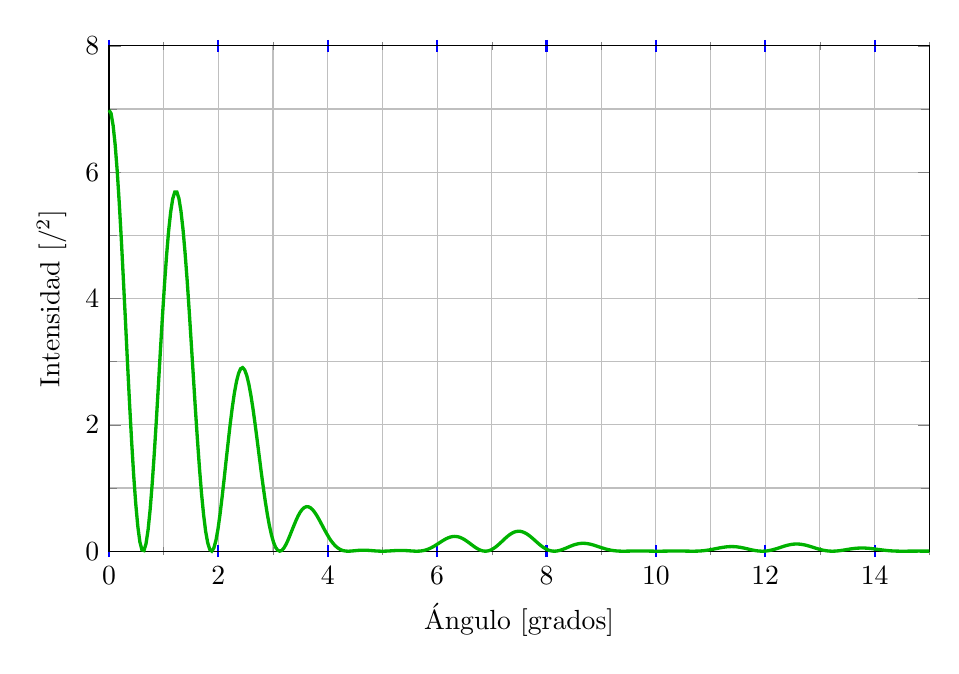
\begin{tikzpicture}[scale=1]
    \begin{axis}[
                 every major x tick/.append style={thick,blue},
                 clip=false,
                 grid=both,
                 minor x tick num=1,        %un minor tick es decir 0.5
                 minor y tick num=1,
                 xmin=0, xmax=15,           %min y max para los ejes, NO PARA EL DOMINIO
                 ymin=0, ymax=8,
                 %axis y line=center,        %alinea el eje al centro de la figura
                 %axis x line=middle,        %sino pone 2 ejes x
                 xtick  align=center,
                 xlabel={Ángulo~[grados]},
                 ylabel={Intensidad~[$\si{\milli\watt/\metre^2}$]},
                 width=12cm,
                 height=8cm
                ];
    \addplot [color=green!70!black, very thick] [samples= 400, domain=0.001:15]  {7*(cos(180*sin(x)*4/sin(5))*sin(180*sin(x)*1/sin(5))/(pi*sin(x)*1/sin(5)))^2};
    \end{axis}
  \end{tikzpicture}
  \captionof{figure}{Problema \ref{p:P245}\label{f:P245}}
\end{center}
%
\pma{\label{p:P267}
Un haz de luz de longitud de onda (en el vacío) $\lambda_0= 500$~nm incide sobre una placa con dos rendijas, separadas entre sí una distancia $d = 25 \mu$m y de ancho $a = \frac15 d$. La placa se encuentra en la división entre dos medios de índice de refracción $n_1 = 1.20$ y $n_2 = 1.28$, respectivamente. Al hacer incidir el haz con un ángulo $\theta_i$, se observa que el patrón de intensidades se desplaza 30 franjas respecto de la situación con incidencia normal. La pantalla de observación está ubicada a $1$~m de distancia de la placa y está centrada respecto del eje del sistema. \textit{a}) Calcule el ángulo de incidencia $\theta_i$. \textit{b}) ¿A qué distancia del eje del sistema se encuentra el centro de la campana principal de difracción? \textit{c}) Calcule la irradiancia en el centro de la pantalla.\\
\rta{.95}{\textit{a}) $\theta_i=30$º; \textit{b}) $53$~cm; \textit{c}) $I=0$}}
%
\pma{\label{p:P305}
Un haz de luz de longitud de onda (en el vacío) $\lambda_0= 600$~nm incide con un ángulo de $0.967$º sobre una placa que contiene dos rendijas de $20\,\mu$m de ancho y separadas $80\,\mu$m.  Se observa el patrón de interferencia en una pantalla situada a 1 m de la placa con las rendijas. \textit{a}) ¿Cuánto mide la interfranja?
\textit{b}) Calcule la intensidad que se registra en el centro de la pantalla, sabiendo que desde cada rendija sale luz con $5$~W/m\textsuperscript{2} de intensidad.\\
\rta{.95}{\textit{a}) $7.5$~mm; \textit{b}) $3.08$~W/m\textsuperscript{2}}}